\documentclass[english,a4paper,onepage, 10pt]{scrbook}

\usepackage[T1]{fontenc}
\usepackage[utf8]{inputenc}
\usepackage{babel}
\pagestyle{headings}
\setcounter{tocdepth}{3}
\setlength\parskip{\medskipamount}
\setlength\parindent{0pt}
\setlength{\unitlength}{1cm}
\addtolength{\textheight}{2cm}
\usepackage{multicol}
\usepackage{lscape}

\usepackage{graphicx}
\usepackage{ae}
\usepackage{aecompl}
\usepackage{amssymb}
\usepackage{amsmath}
\usepackage{bookman}
\usepackage{multicol}
\usepackage{gensymb}
\usepackage{listings}
\usepackage{pdfpages}
% For astrology signs
\usepackage{wasysym}
\usepackage{marvosym}


\usepackage{geometry}
%\areaset[-2cm]{18cm}{26cm}

%\linespread{0.9}


\begin{document}

\newcommand{\tavla}[1]{\reversemarginpar{ \rule[-10mm]{0.1mm}{#1cm}}}
\newcommand{\svarsrad}{\begin{flushright} \rule{7cm}{0.2mm} \end{flushright}}
\newcommand{\asm}[1]{\texttt{\textbf{#1}}}

\newcommand{\startex}[1]{\textbf{Example}\begin{quote}#1\end{quote}}
\newcommand{\slutex}{\begin{flushright}\rule{1ex}{1ex}\end{flushright}}


\title{Sun's position for navigation with DM15/HP-15c\\{}Manual\\{}}

\author{Michael Josefsson}
\date{\today}
\maketitle
\tableofcontents

\addtolength{\evensidemargin}{-2.0cm}
\addtolength{\oddsidemargin}{2.0cm}
\setcounter{chapter}{1}

\newpage
\section{Overview}

The handheld calculator DM15 (a HP-15c look-a-like with more memory) can be used for determining the sun's position with precision enough for celestial navigation purposes. The accompanying program, listed in the Appendix, constitutes a handy tool for either finding the \emph{Nautical Almanac}'s entries GHA (\emph{Greenwich Hour Angle}) and Declination, or --- with AP (\emph{Assumed Position}) --- directly calculate the sun's Altitude \emph{Hc} and Azimuth \emph{Az} for this position.

The algorithm relies on pure Keplerian motion of the sun. No planetary perturbations are taken into account. Resulting angular accuracy is about 1 minute of arc, which is adequate for general navigation at sea.

\section{General notes} 

Before use, notice that: 

\begin{itemize}
\item All times entered are UT (''GMT'') even if observer's longitude is not the prime meridian. Of course, local hour angles take longitude into consideration, but all times are still UT. Time format is $hh.mmss$, where $mm$ and $ss$ must be two-digit numbers.


\item The program makes use of the calculator's internal decimal to degrees, minutes and seconds routines both for \textbf{entry} and \textbf{displayed result}. In navigation a more common format of degrees, minutes and tenths of a minute is used. That conversion, if needed, is readily done by dividing the arc-seconds number or multiplying the minute's decimal by 6.

\startex{Convert angle in $ddd.mmss$ to $ddd.mm{\cdot}t$}

 $98\degree\, 26'\, 12''$, entered as \asm{98.2612},  is $98\degree\, 26{\cdot}2'$ where $12''/6=2$\\
 $98\degree\, 26'\, 43''$, entered as \asm{98.2643}, is $98\degree\, 26{\cdot}7'$ where $43''/6\approx7$
 \slutex
 
\startex{Convert angle in $ddd.mm{\cdot}t$ to $ddd.mmss$}

 $14\degree\, 7{\cdot}3'$  is $14\degree\, 7'\, 18''$ where $3 \cdot 6=18$\\
 $277\degree\, 4{\cdot}5'$  is $277\degree\, 4{\cdot}30'$ where $5 \cdot 6=30$
 \slutex
 
\end{itemize}
 

\section{Public routines} 

Full use of the program entails the following routines where \textbf{\textsf{A--E}} are main functionality and \textbf{\textsf{.0, 4, 5, 9}} are utilities. Their use is described in this document. 

\begin{center}
\begin{tabular}{ll}
Button & Function \\
\hline
\textbf{\textsf{A}} & Date for \Aries\, hour angle at UT=0h\\
\textbf{\textsf{B}} & Time for Sun Altitude and Azimuth \\
\textbf{\textsf{C}} & SHA and declination for \emph{own object} \\
\textbf{\textsf{D}} & GMT $\rightarrow$ \emph{own object}'s Altitude and Azimuth \\
\textbf{\textsf{E}} & GMT $\rightarrow$ GHA \Aries\, and LHA \Aries\,\\

\textbf{\textsf{.0}} & GHA, time and declination $\rightarrow$ Altitude and Azimuth\\
\textbf{\textsf{.4}} & GHA, $\delta T$, \emph{v}  $\rightarrow$ GHA for newtime\\

\textbf{\textsf{.5}} & After \textbf{\textsf{B}} $\rightarrow$ GHA and declination\\

& (mimicks a \emph{Nautical Almanac} entry)\\
\textbf{\textsf{.9}} & True altitude $\rightarrow$ Apparent Altitude\\

\end{tabular}
\end{center}

\section{Usage for Sun}
 
The program's main purpose is to give altitude and azimuth for the sun. This requires an \emph{Assumed Position}, date and time.

\subsection{First set AP (\emph{Assumed Position})} An AP is entered in registers \asm{\textbf{8}} and \asm{\textbf{.8}} before any calculations can be peformed.

\startex{Entering AP.} A location of Lat N$58\degree\, 34'$, Long E$14\degree\, 34'\,12''$ is entered into registers \asm{\textbf{8}} and \asm{\textbf{.8}}:

\begin{tabular}{ccr|lc}
Data & Format & Key & &Display shows\\
\asm{58.3400} & $\pm dd.mmss$ & g ->H &\asm{STO 8} &\asm{58.5667}\\
\asm{14.3412} & $\pm dd.mmss$ & g ->H &\asm{STO .8} &\asm{14.5700}\\
\end{tabular}

East and North are positive, West and South are negative. \\The position is permanently stored until manually changed and need only be set once.
\slutex

\newpage

\subsection{Then set the date} Each day has its own parameters and require the \asm{\textbf{A}}-routine to be run each new day.

\startex{Entering the date.} Enter June 12th 2022, i.e. year 2022, month 6 and day 12

\begin{tabular}{ccr|lc}
Data       & Format      & Key & &Display shows\\
\asm{2022} &  $YYYY$   & ENTER &&\asm{2022.0000}\\
\asm{6} &  $mm$   & ENTER &&\asm{6.0000}\\

\asm{12} &  $dd$   & f \asm{\textbf{A}} &&\asm{260.1816} ($260\degree\, 18'\,17''=260\degree\, 18{\cdot}3'$, GHA \Aries\, at 0h)\\
\end{tabular}

This is only necessary once for each day.

\slutex 

\subsection{Finally enter time in GMT for Altitude and Azimuth} Next the sun's coordinates for time of date UT/GMT can be  calculated.

\startex{Find sun's Hc and Az for UT 09h 54m 48s. Date entered as above.} Enter time in format $hh.mmss$ then use routine \asm{\textbf{B}}.

\begin{tabular}{ccr|lc}
Data       & Format      & Key & &Display shows\\
\asm{9.5448} &  $hh.mmss$   & f \asm{\textbf{B}} &&\asm{52.3845} ( Hc = $52\degree\, 38'\,45''$ )\\
&    &  \asm{\textbf{x<>y}} &&\asm{154.1140} ( Az = $154\degree\, 11'\,40''$ )\\
\end{tabular}

\textbf{Result:} Hc = $52\degree\, 38{\cdot}7'$, Az = $154\degree$

A new time can be entered directly. For example, also find sun's Hc and Az a few minutes later at UT 10h 02m 30s. 

\begin{tabular}{ccr|lc}
Data       & Format      & Key & &Display shows\\
\asm{10.0230} &  $hh.mmss$   & f \asm{\textbf{B}} &&\asm{53.0338} ( Hc = $53\degree\, 03'\,38''$ )\\
&    &  \asm{\textbf{x<>y}} &&\asm{157.0236} ( Az = $157\degree\, 2'\,36''$ )\\
\end{tabular}

\textbf{Result:} Hc = $53\degree\, 03{\cdot}6'$, Az = $157\degree$

\slutex


\subsection{Calculate Sun's GHA and Declination} 
If wanted the program can also produce values for GHA and Declination imitating the \emph{Nautical Almanac}.

\startex{Find GHA and decl for 10h on June 12th 2023} The date must be set as above. Now enter time to get Hc and Az if wanted. Or ignore the output and use \asm{\textbf{GSB .5}} to get GHA and decl:

\begin{tabular}{ccr|lc}
Data       & Format      & Key  &Display shows\\
\asm{10.0000} &  $hh.mmss$   & f \asm{\textbf{B}} &\asm{52.5508} ( Hc = $52\degree\, 55'\,08''$, ignore )\\
&    &  \asm{\textbf{GSB .5}} &\asm{330.0248} ( GHA = $330\degree\, 2'\,48''$ )\\
&    &  \asm{\textbf{x<>y}} &\asm{23.0901} ( Decl = N$23\degree\, 09'\,01''$ )\\
\end{tabular}

\textbf{Result:} GHA = $330\degree\, 2{\cdot}8'$, Decl = N$23\degree\, 09{\cdot}0'$ (\emph{Nautical Almanac} gives $330\degree\, 2{\cdot}8'$ and N$23\degree\, 8{\cdot}8'$).

GHA and Decl can of course be calculated for any other time during the day in the same manner. 
%\slutex




\vspace{-5mm}

\section{SHA and Declination $\rightarrow$ Altitude and Azimuth}

The coordinates of a celestial object, for example a star, are given as SHA (\emph{Sidereal Hour Angle}) and Declination.\footnote{Right Ascension can be entered as $\alpha=360 - SHA$ if needed.}

\startex{Coordinates of \emph{Vega} (SHA $80\degree\, 34{\cdot}3'$, declination $38\degree\, 48{\cdot}2'$) are entered}


\begin{tabular}{ccr|lc}
Data       & Format      & Key & Display shows\\
\asm{80.3418} &  $ddd.mmss$   & ENTER &\asm{80.3418}&\\
\asm{38.4812} &  $ddd.mmss$   & f \asm{\textbf{C}} & \asm{279.4283} (RA in decimal degrees as a bonus)\\
\end{tabular}

Now find \emph{Vega}'s calculated position for UT = 23h 02m 10s on June 12th 2023 already entered above.

\begin{tabular}{ccr|lc}
Data       & Format      & Key & Display shows\\
\asm{23.0210} &  $hh.mmss$   & f \asm{\textbf{D}} &\asm{67.0015} ( Hc = $67\degree\, 00'\,15''$ ) \\
&    &  \asm{\textbf{x<>y}} &\asm{141.1224} ( Az = $141\degree\, 12'\,24''$ )\\
\\
\end{tabular}

\textbf{Result:} Vega can be expected at \emph{Hc} = $67\degree\, 0{\cdot}2'$ and \emph{Zn} =  $141\degree$. Set the sextant for $67\degree$ and search for it in south-east.


\section{Date and time $\rightarrow$ GHA \Aries\,  and LHA \Aries\,} 

Find GHA \Aries\, on 4 October 2022 at 7h 57m 20s. Also find LHA \Aries\, longitude in \asm{.8} (E$14\degree\, 34'\,12''$  as before).

\begin{tabular}{ccr|lc}
Data       & Format      & Key & Display shows\\
\hline
\asm{2022} &  $YYYY$   & ENTER &\asm{2022.0000}\\
\asm{10} &  $mm$   & ENTER &\asm{10.0000}\\
\asm{4} &  $dd$   & f \asm{\textbf{A}} &\asm{12.4006} ($12\degree\, 40'\,6''$, GHA \Aries\, at 0h)\\
\asm{7.5720} &  $hh.mmss$   & f \asm{\textbf{E}} &\asm{132.1942} ( GHA \Aries\, = $132\degree\, 19'\,42''$ ) \\
&    &  \asm{\textbf{x<>y}} &\asm{146.5354} ( LHA \Aries\, = $146\degree\, 53'\,54''$ )\\
\end{tabular}

\section{.4, GHA, $\Delta T$, \emph{v}  $\rightarrow$ GHA for time $+\Delta T$} 

This routine replaces the GHA part of the \emph{Sun and Planets}-section\footnote{Will not work for Moon or Aries.} of \textsc{Increments and Corrections} as found in the \emph{Nautical Almanac}. It (linearly) interpolates a future GHA given 

\begin{itemize}
\item a current GHA, 
\item a time difference from this GHA and 
\item \emph{v} as read from the \emph{Nautical Almanac}.
\end{itemize}

\startex{Given that the GHA is $110\degree\, 34{\cdot}3'$ at 17h. What is the GHA at 17h 23m 47s? \emph{v}-value is 2.4 as read from the NA.}

\begin{tabular}{rcr|lc}
Data       & Format      & Key & Display shows\\
\hline
\asm{110.3418} &  $ddd.mmss$   & ENTER &\asm{110.3418}\\
\asm{0.2347} &  $hh.mmss$   & ENTER &\asm{0.2347}\\
\asm{2.4} &  $min.tenths$   & \asm{\textbf{GSB .4}} &\asm{116.3200} ($116\degree\, 32'\,00''$, GHA at 17h 23m 47s)\\
\end{tabular}

\section{.3, Declination, $\Delta T$, \emph{d}  $\rightarrow$ Declination for time $+\Delta T$} 

This routine replaces the \emph{d-corr} part of \textsc{Increments and Corrections} as found in the \emph{Nautical Almanac}. It (linearly) interpolates a future Declination given 

\begin{itemize}
\item a current declination at time $T$, 
\item a time difference, $\Delta T$, from this and 
\item \emph{d} as read from the \emph{Nautical Almanac}.
\end{itemize}

Beware of signs. 

Decreasing positive declinations -> d negative (numerically smaller)

Decreasing negative declinations -> d positive (numerically larger)



%\startex{Given that the GHA is $110\degree\, 34{\cdot}3'$ at 17h. What is the GHA at 17h 23m 47s? \emph{v}-value is 2.4 as read from the NA.}
%
%\begin{tabular}{rcr|lc}
%Data       & Format      & Key & Display shows\\
%\hline
%\asm{110.3418} &  $ddd.mmss$   & ENTER &\asm{110.3418}\\
%\asm{0.2347} &  $hh.mmss$   & ENTER &\asm{0.2347}\\
%\asm{2.4} &  $min.tenths$   & \asm{\textbf{GSB .4}} &\asm{116.3200} ($116\degree\, 32'\,00''$, GHA at 17h 23m 47s)\\
%\end{tabular}


\section{.0, GHA and Declination $\rightarrow$ Altitude and Azimuth} 

When coordinates are given as GHA (\emph{Greenwich Hour Angle}) and Declination, as is the case for the planets and Moon listed in NA,  proceed as follows. As GHA changes continuously during the day a time is also required.

\startex{Coordinates of \emph{Sun} as from \emph{Nautical Almanac} above are GHA $330\degree\, 2{\cdot}8'$, declination N$23\degree\, 8{\cdot}8'$ at 10h.}


\begin{tabular}{ccr|lc}
Data       & Format      & Key & Display shows\\
\asm{330.0248} &  $ddd.mmss$   & \asm{ENTER} &\asm{330.0248}&\\
\asm{10.0000} &  $ddd.mmss$   & \asm{GSB .0} &\asm{279.3413}, ignore&\\
\asm{23.0848} &  $ddd.mmss$   & \asm{R/S} & \asm{52.5455}  ( Hc = $52\degree\, 54'\,55''$ ) 
\\
&    &  \asm{\textbf{x<>y}} &\asm{156.0821} ( Az = $156\degree\, 08'\,21''$ )\\

\end{tabular}

\textbf{Result:} The \emph{Sun} is expected at a height of $52\degree\, 54{\cdot}9'$ and in a direction of $156\degree$.\footnote{Compare these results with the direct method above ($52\degree\, 54'\,55''$ vs $52\degree\, 55'\,08''$ and $156\degree\, 08'\,16''$ vs $156\degree\, 08'\,21''$). Pretty close but not exactly the same. }


\section{.9, True Altitude $\rightarrow$ Apparent Altitude} 


The calculated altitude of any object is the True Altitude. Due to refraction the object will appear at a slightly higher altitude, its Apparent Altitude. This routine adds the correct small amount of refraction correction.\footnote{S\ae mann's formula is used.}

\startex{Calculated altitude of a star is $17\degree\, 45'\,00''$. What is the star's Apparent Altitude?}

\begin{tabular}{ccr|lc}
Data       & Format      & Key & Display shows\\
\asm{17.4500} &  $ddd.mmss$   & \asm{GSB .9} &\asm{17.4806} $H_{app}$ = $17\degree\, 48'\,06''$ &\\
              &  $$   & \asm{x<>y} &\asm{0.0306}, the increment added, $03'\,06''$&\\
\end{tabular}

\textbf{Note:} With negligible error this routine can also be used to find the refraction correction as in \textsc{altitude correction tables} in \emph{Nautical Almanac}. 

\startex{Measured altitude of a star is $17\degree\, 48'\,06''$. What is the star's True Altitude? (Inverse example of above)}

\begin{tabular}{ccr|lc}
Data       & Format      & Key & Display shows\\
\asm{17.4806} &  $ddd.mmss$   & \asm{GSB .9} &\asm{17.5112}, ignore result &\\
              &  $$   & \asm{x<>y} &\asm{0.0306}, the increment to subtract, $03'\,06''$&\\
\end{tabular}

This value matches closely the \emph{Nautical Almanac}'s value of $-03'$.

\section{Use as \emph{Sight Reduction Table}} 

The program can also solve the navigational triangle and be used as a (Ho-214/Ho-229 etc) \emph{Sight Reduction Table} replacement. To solve the triangle  AP latitude, object's declination and hour angle needs to be entered.

AP latitude is entered in register \asm{8} as before, declination is set via \textbf{\textsf{C}} and hour angle is entered into register \asm{.2}. The hour angle is positive if westward.

\startex{Find Hc and Az as in Ho-214} Assume longitude $58\degree$~N, Declination $8\degree\, 30'$ and an hour angle of $54\degree$ (object to the west of observer).

\begin{tabular}{ccr|lc}
Data       & Format      & Key & Display shows\\
\hline
\asm{58} &  $dd.mmss$   & \asm{STO 8} &\asm{58.0000}\\
\asm{8.3000} &  $dd.mmss$   & \textbf{\textsf{C}} &\asm{8.5000}\\
\asm{54}     &  $dd.mmss$   & g ->H & \asm{54.0000}\\
             &              & \asm{STO .2} & \asm{54.0000}\\
             &              & \asm{GSB 7} & \asm{25.4102} ( Hc = $25\degree\, 41'\,02''$)\\
             &              &  \asm{\textbf{x<>y}} &\asm{242.3616} ( Az = $242\degree\, 36'\,16''$ = 242.60\degree)\\
\end{tabular}

Ho-214 gives Alt. = $25\degree\, 41{\cdot}0'$ and  Az. = $117.4\degree$. Where true azimuth is $360-117.4=242.6\degree$. 




\section{Program and information}
\subsection{Register usage}
The lower registers \asm{r0..r7} are used by the calculator's statistics functions and are not \emph{permanently} used by this program. They \emph{are} used however for intermediate results via the normal operating sequences \textbf{\textsf{A-B}} or \textbf{\textsf{A-C-D}} or \textbf{\textsf{A-E}}.

In short: Use \asm{r0..r7} as you wish but they will be altered by \textbf{\textsf{A}}.

\subsection{Program installation}

For a fresh install of the program perform steps 1--6 below.

\begin{enumerate}

\item Make space on the DM15 for program and registers:
\begin{itemize}
 \item Enter \asm{\textbf{21 f DIM (i)}}  
 
 \item Double check:  \asm{\textbf{g MEM}} should read \asm{21.209}
 \end{itemize}
 
 \item In \textsf{HP-15C/Preferences/DM15 menu}: Select \textsf{229} as Number of registers.
 
 \item \textsf{File/Open Program}: file.15c
 
 \item Write program to DM15.
 \begin{itemize}

 \item On device enable serial communication (hold C while pressing ON-button) 
 \item \textsf{File/Write DM15}
 \end{itemize}
 \item Before use a number of constants must be entered in the following registers:
  
 \begin{tabular}{cl}
 Register & Constant\\
 \hline
 \asm{.3} & \asm{\textbf{279.4055638}}\\
 \asm{.4} &  \asm{\textbf{283.3328093}}\\
 \asm{.5} &  \asm{\textbf{1.016860112}}\\
 \asm{.6} &  \asm{\textbf{23.44188400}}\\
 \asm{.7} &  \asm{\textbf{0.002737909}}, (1/365.2422)\\
 \hline
 \end{tabular}
 
 \item That's it. Now the samples in this document should give the expected results.
\end{enumerate}

\subsection{Program listing}

\lstset{basicstyle=\fontsize{10}{10}\selectfont\ttfamily, tabsize=4}
Note: In the listing below some minor self explanatory key appearances have changed.  \asm{SIN}$^{-1}$ is replaced with \asm{ASIN} etc, \asm{x}$\leftrightarrow$\asm{y} is \asm{x<>y} and \asm{R}$\downarrow$ is \asm{Rv}.
\begin{multicols}{2}
\begin{lstlisting}
   000 {             } 
   001 { 42 21 48  8 } f LBL .8
   002 {           3 } 3
   003 {           6 } 6
   004 {           0 } 0
   005 {       43 32 } g RTN
   006 {    42 21  4 } f LBL 4
   007 {          23 } SIN
   008 {          34 } x<>y
   009 {          23 } SIN
   010 {    22 48  6 } GTO .6
   011 {    42 21  5 } f LBL 5
   012 {          24 } COS
   013 {          34 } x<>y
   014 {          24 } COS
   015 {    22 48  6 } GTO .6
   016 {    42 21  2 } f LBL 2
   017 {    32 48  8 } GSB .8
   018 {          10 } /
   019 {       42 44 } f FRAC
   020 {    43 30  1 } g TEST x>0
   021 {       22  3 } GTO 3
   022 {           1 } 1
   023 {          40 } +
   024 {    42 21  3 } f LBL 3
   025 {    32 48  8 } GSB .8
   026 { 42 21 48  6 } f LBL .6
   027 {          20 } *
   028 {       43 32 } g RTN
   029 { 42 21 48  2 } f LBL .2
   030 {           1 } 1
   031 {           5 } 5
   032 {    22 48  6 } GTO .6
   033 {    42 21 12 } f LBL B
   034 {       32 15 } GSB E
   035 {       45  6 } RCL 6
   036 {           2 } 2
   037 {           4 } 4
   038 {           5 } 5
   039 {           9 } 9
   040 {           9 } 9
   041 {           4 } 4
   042 {           4 } 4
   043 {          48 } .
   044 {           5 } 5
   045 {          30 } -
   046 {       45  4 } RCL 4
   047 {           2 } 2
   048 {           4 } 4
   049 {          10 } /
   050 {          40 } +
   051 {    45 48  7 } RCL .7
   052 {    32 48  8 } GSB .8
   053 {          20 } *
   054 {          20 } *
   055 {    45 48  3 } RCL .3
   056 {          40 } +
   057 {    45 48  4 } RCL .4
   058 {          30 } -
   059 {       42  3 } f ->RAD
   060 {       44  9 } STO 9
   061 {       43  8 } g RAD
   062 {          36 } ENTER
   063 {           1 } 1
   064 {           0 } 0
   065 {    42  7  9 } f FIX 9
   066 {    42 10  8 } f SOLVE 8
   067 {    42  7  4 } f FIX 4
   068 {           2 } 2
   069 {          10 } /
   070 {          25 } TAN
   071 {    45 48  5 } RCL .5
   072 {          20 } *
   073 {       43 25 } g ATAN
   074 {           2 } 2
   075 {          20 } *
   076 {       43  3 } g ->DEG
   077 {       43  7 } g DEG
   078 {    45 48  4 } RCL .4
   079 {          40 } +
   080 {    44 48  0 } STO .0
   081 {    45 48  0 } RCL .0
   082 {          23 } SIN
   083 {    45 48  6 } RCL .6
   084 {          24 } COS
   085 {          20 } *
   086 {    45 48  0 } RCL .0
   087 {          24 } COS
   088 {       43  1 } g ->P
   089 {          33 } Rv
   090 {       44  9 } STO 9
   091 {    45 48  0 } RCL .0
   092 {          23 } SIN
   093 {    45 48  6 } RCL .6
   094 {          23 } SIN
   095 {          20 } *
   096 {       43 23 } g ASIN
   097 {    44 48  0 } STO .0
   098 {       45  9 } RCL 9
   099 { 42 21 48  1 } f LBL .1
   100 {       45  5 } RCL 5
   101 {    32 48  8 } GSB .8
   102 {       45  9 } RCL 9
   103 {          30 } -
   104 {          40 } +
   105 {       32  2 } GSB 2
   106 {    44 48  2 } STO .2
   107 {       32  7 } GSB 7
   108 {       43 32 } g RTN
   109 {    42 21  7 } f LBL 7
   110 {    45 48  2 } RCL .2
   111 {          24 } COS
   112 {       45  8 } RCL 8
   113 {    45 48  0 } RCL .0
   114 {       32  5 } GSB 5
   115 {          20 } *
   116 {    45 48  0 } RCL .0
   117 {       45  8 } RCL 8
   118 {       32  4 } GSB 4
   119 {          40 } +
   120 {       43 23 } g ASIN
   121 {          36 } ENTER
   122 {          36 } ENTER
   123 {    44 48  1 } STO .1
   124 {       45  8 } RCL 8
   125 {       32  4 } GSB 4
   126 {          16 } CHS
   127 {    45 48  0 } RCL .0
   128 {          23 } SIN
   129 {          40 } +
   130 {          34 } x<>y
   131 {       45  8 } RCL 8
   132 {       32  5 } GSB 5
   133 {          10 } /
   134 {       43 24 } g ACOS
   135 { 42  4 48  2 } f X<>.2
   136 {          23 } SIN
   137 {    43 30  2 } g TEST x<0
   138 {       22  6 } GTO 6
   139 {    32 48  8 } GSB .8
   140 {    45 48  2 } RCL .2
   141 {          30 } -
   142 {    44 48  2 } STO .2
   143 {    42 21  6 } f LBL 6
   144 {    45 48  1 } RCL .1
   145 {    45 48  2 } RCL .2
   146 {       22  9 } GTO 9
   147 {    42 21  8 } f LBL 8
   148 {          23 } SIN
   149 {          48 } .
   150 {           0 } 0
   151 {           1 } 1
   152 {           6 } 6
   153 {           7 } 7
   154 {           1 } 1
   155 {           8 } 8
   156 {          20 } *
   157 {          16 } CHS
   158 {          40 } +
   159 {       45  9 } RCL 9
   160 {          30 } -
   161 {       43 32 } g RTN
   162 {    42 21 13 } f LBL C
   163 {       43  2 } g ->H
   164 {    44 48  0 } STO .0
   165 {          33 } Rv
   166 {       43  2 } g ->H
   167 {    32 48  8 } GSB .8
   168 {          34 } x<>y
   169 {          30 } -
   170 {       44  9 } STO 9
   171 {       43 32 } g RTN
   172 {    42 21 15 } f LBL E
   173 {       43  2 } g ->H
   174 {       44  4 } STO 4
   175 {    45 48  7 } RCL .7
   176 {           1 } 1
   177 {          40 } +
   178 {          20 } *
   179 {    32 48  2 } GSB .2
   180 {       45  1 } RCL 1
   181 {          40 } +
   182 {          36 } ENTER
   183 {          36 } ENTER
   184 {    45 48  8 } RCL .8
   185 {          40 } +
   186 {       32  2 } GSB 2
   187 {       44  5 } STO 5
   188 {          34 } x<>y
   189 {       32  2 } GSB 2
   190 {          34 } x<>y
   191 {    42 21  9 } f LBL 9
   192 {       42  2 } f ->H.MS
   193 {          34 } x<>y
   194 {       42  2 } f ->H.MS
   195 {       43 32 } g RTN
   196 {    42 21  0 } f LBL 0
   197 {           1 } 1
   198 {          36 } ENTER
   199 {           0 } 0
   200 {       32  1 } GSB 1
   201 {           2 } 2
   202 {           4 } 4
   203 {           1 } 1
   204 {           5 } 5
   205 {           0 } 0
   206 {           2 } 2
   207 {           0 } 0
   208 {          30 } -
   209 {           3 } 3
   210 {           6 } 6
   211 {           5 } 5
   212 {           2 } 2
   213 {           5 } 5
   214 {          10 } /
   215 {          36 } ENTER
   216 {          36 } ENTER
   217 {          48 } .
   218 {           0 } 0
   219 {           0 } 0
   220 {           0 } 0
   221 {           0 } 0
   222 {           2 } 2
   223 {           5 } 5
   224 {           8 } 8
   225 {           1 } 1
   226 {          20 } *
   227 {           2 } 2
   228 {           4 } 4
   229 {           0 } 0
   230 {           0 } 0
   231 {          48 } .
   232 {           0 } 0
   233 {           5 } 5
   234 {           1 } 1
   235 {           2 } 2
   236 {           6 } 6
   237 {           2 } 2
   238 {          40 } +
   239 {          20 } *
   240 {           6 } 6
   241 {          48 } .
   242 {           6 } 6
   243 {           4 } 4
   244 {           6 } 6
   245 {           0 } 0
   246 {           6 } 6
   247 {           5 } 5
   248 {           6 } 6
   249 {          40 } +
   250 {    32 48  2 } GSB .2
   251 {       32  2 } GSB 2
   252 {       44  3 } STO 3
   253 {       45  6 } RCL 6
   254 {       44  0 } STO 0
   255 {       43 32 } g RTN
   256 {    42 21 11 } f LBL A
   257 {       44  4 } STO 4
   258 {          33 } Rv
   259 {       44  5 } STO 5
   260 {          33 } Rv
   261 {       32  0 } GSB 0
   262 {       45  1 } RCL 1
   263 {       45  5 } RCL 5
   264 {       45  4 } RCL 4
   265 {       32  1 } GSB 1
   266 {       45  0 } RCL 0
   267 {          30 } -
   268 {    45 48  7 } RCL .7
   269 {    32 48  8 } GSB .8
   270 {          20 } *
   271 {          20 } *
   272 {       45  3 } RCL 3
   273 {          40 } +
   274 {       32  2 } GSB 2
   275 {       44  1 } STO 1
   276 {       42  2 } f ->H.MS
   277 {       43 32 } g RTN
   278 {    42 21  1 } f LBL 1
   279 {           1 } 1
   280 {           7 } 7
   281 {           2 } 2
   282 {           1 } 1
   283 {           0 } 0
   284 {           1 } 1
   285 {           3 } 3
   286 {          48 } .
   287 {           5 } 5
   288 {          40 } +
   289 {          34 } x<>y
   290 {       44  1 } STO 1
   291 {           2 } 2
   292 {           7 } 7
   293 {           5 } 5
   294 {          20 } *
   295 {           9 } 9
   296 {          10 } /
   297 {       43 44 } g INT
   298 {          40 } +
   299 {          34 } x<>y
   300 {          36 } ENTER
   301 {    42  4  1 } f X<>1
   302 {           9 } 9
   303 {          40 } +
   304 {           1 } 1
   305 {           2 } 2
   306 {          10 } /
   307 {       43 44 } g INT
   308 {          40 } +
   309 {           7 } 7
   310 {          20 } *
   311 {           4 } 4
   312 {          10 } /
   313 {       43 44 } g INT
   314 {          16 } CHS
   315 {          40 } +
   316 {       45  1 } RCL 1
   317 {           3 } 3
   318 {           6 } 6
   319 {           7 } 7
   320 {          20 } *
   321 {          40 } +
   322 {       44  6 } STO 6
   323 {       43 32 } g RTN
   324 {    42 21 14 } f LBL D
   325 {       32 15 } GSB E
   326 {    32 48  1 } GSB .1
   327 {       43 32 } g RTN
   328 { 42 21 48  5 } f LBL .5
   329 {       45  5 } RCL 5
   330 {    45 48  8 } RCL .8
   331 {          30 } -
   332 {    32 48  8 } GSB .8
   333 {       45  9 } RCL 9
   334 {          30 } -
   335 {          40 } +
   336 {       32  2 } GSB 2
   337 {    45 48  0 } RCL .0
   338 {       22  9 } GTO 9
   339 { 42 21 48  0 } f LBL .0
   340 {       32 15 } GSB E
   341 {       43  2 } g ->H
   342 {       43 33 } g R^
   343 {       43  2 } g ->H
   344 {          34 } x<>y
   345 {          30 } -
   346 {       42  2 } f ->H.MS
   347 {          31 } R/S
   348 {       32 13 } GSB C
   349 {       45  4 } RCL 4
   350 {       42  2 } f ->H.MS
   351 {       32 14 } GSB D
   352 {       43 32 } g RTN
\end{lstlisting}
\end{multicols}
\newpage
\appendix
\begin{landscape}
\Large

\section*{Short summary}
\begin{tabular}{rcl}
 Format & Button  &Function \\
\hline

$YYYY\,\, MM\, DD$             & \textbf{\textsf{A}} & Initialize with date\\
$hh.mmss$                & \textbf{\textsf{B}} & Get Sun's Altitude for Time, x<>y Azimuth\\
$ddd.mmss$ $\pm decl$ & \textbf{\textsf{C}} & Enter own objects coordinates\\
$hh.mmss$                & \textbf{\textsf{D}} & Own object's Altitude for Time, x<>y Azimuth\\
 $hh.mmss$                & \textbf{\textsf{E}} & GHA \Aries\,, x<>y for LHA \Aries\,\\
\hline
 $ddd.mmss$ $hh.mmss$   & \textbf{\textsf{GSB .0}} & GHA, x<>y for Azimuth of Sun\\
  $dd.mmss$    & \textbf{\textsf{R/S}}  &Object's Altitude for Time, x<>y Azimuth\\
\hline
 $\pm dd.mmss$ $0.mmss$  $d$  & \textbf{\textsf{GSB .3}} & Decl for Time \\
  $\pm ddd.mmss$ $0.mmss$  $v$  & \textbf{\textsf{GSB .4}} & GHA for Time \\

  After \textbf{\textsf{A}}   & \textbf{\textsf{GSB .5}} & Sun's GHA, x<>y Declination\\
 $dd.mmss$  & \textbf{\textsf{GSB .9}} & Apparent altitude, x<>y refr corr$^n$ used (in ')\\
\end{tabular}
\end{landscape}
%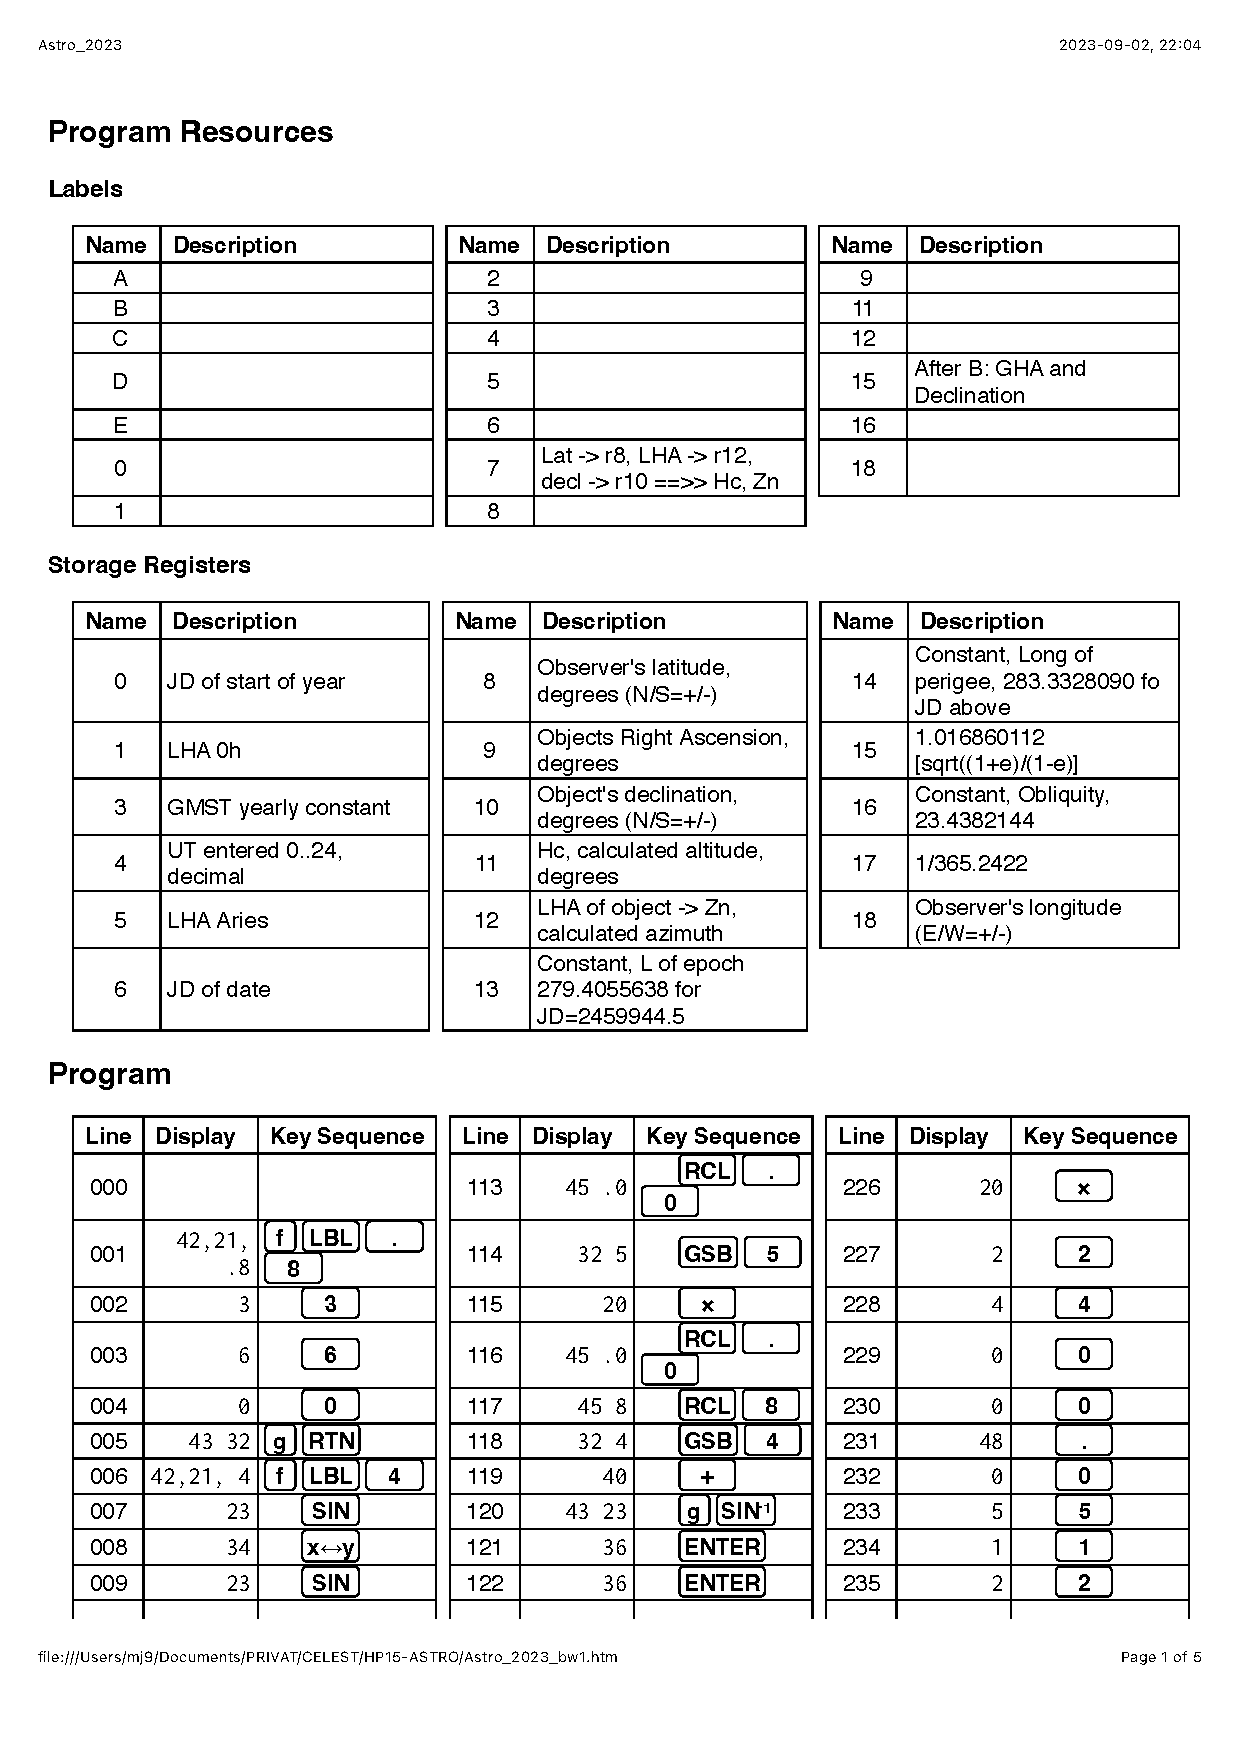
\includepdf[pages={1-5}, scale=0.9]{Astro_2023_bw.pdf}
\end{document}

